\documentclass[japanese,dvipdfmx]{jbook}

\usepackage{master}
%%%%%%%%%%%%%%%%%%%%%%%%%%%%%%%%%%%%%%%%%%%%%%%%%%%%%%%%%%%%%%%%
% User-defined Macro
%%%%%%%%%%%%%%%%%%%%%%%%%%%%%%%%%%%%%%%%%%%%%%%%%%%%%%%%%%%%%%%%
\newcommand{\compress}{\itemsep0pt\parsep0pt\parskip0pt\partopsep0pt}
% \newcommand{\compress}{\itemsep1pt plus1pt\parsep0pt\parskip0pt}
% \newcommand{\code}[1]{\lstinline[basicstyle=\ttfamily]{#1}}
\newcommand{\gringo}{\textit{gringo}}
\newcommand{\clasp}{\textit{clasp}}
\newcommand{\clingo}{\textit{clingo}}
\newcommand{\teaspoon}{\textit{teaspoon}}
\newcommand{\sat}{\textsf{SAT}}
\newcommand{\unsat}{\textsf{UNSAT}}
% \newcommand{\web}[2]{\href{#1}{#2\ \raisebox{-0.15ex}{\beamergotobutton{Web}}}}
% \newcommand{\doi}[2]{\href{#1}{#2\ \raisebox{-0.15ex}{\beamergotobutton{DOI}}}}
% \newcommand{\weblink}[1]{\web{#1}{#1}}
% \newcommand{\imp}{\mathrel{\Rightarrow}}
% \newcommand{\Iff}{\mathrel{\Leftrightarrow}}
% \newcommand{\mybox}[1]{\fbox{\rule[.2cm]{0cm}{0cm}\mbox{${#1}$}}}
% \newcommand{\mycbox}[2]{\tikz[baseline]\node[fill=#1!10,anchor=base,rounded corners=2pt] () {#2};}
% \newcommand{\naf}[1]{\ensuremath{{\sim\!\!{#1}}}}
% \newcommand{\head}[1]{\ensuremath{\mathit{head}(#1)}}
% \newcommand{\body}[1]{\ensuremath{\mathit{body}(#1)}}
% \newcommand{\atom}[1]{\ensuremath{\mathit{atom}(#1)}}
% \newcommand{\poslits}[1]{\ensuremath{{#1}^+}}
% \newcommand{\neglits}[1]{\ensuremath{{#1}^-}}
% \newcommand{\pbody}[1]{\poslits{\body{#1}}}
% \newcommand{\nbody}[1]{\neglits{\body{#1}}}
% \newcommand{\Cn}[1]{\ensuremath{\mathit{Cn}(#1)}}
% \newcommand{\reduct}[2]{\ensuremath{#1^{#2}}}
% \newcommand{\OK}{\mbox{\textcolor{green}{\Pisymbol{pzd}{52}}}}
% \newcommand{\KO}{\mbox{\textcolor{red}{\Pisymbol{pzd}{56}}}}
% \newcommand{\code}[1]{\lstinline[basicstyle=\ttfamily]{#1}}
% \newcommand{\lw}[1]{\smash{\lower2.ex\hbox{#1}}}
\newcommand{\llw}[1]{\smash{\lower3.ex\hbox{#1}}}

\newenvironment{tableC}{%
  \scriptsize
  \renewcommand{\arraystretch}{0.9}
  \tabcolsep = 0.6mm
  % \begin{tabular}[t]{p{6mm}|rlr|rlr|rlr|rlr|rlr}\hline
  %   \multicolumn{1}{l|}{\llw{問題   }} &
  \begin{tabular}[t]{l|rlr|rlr|rlr|rlr|rlr}\hline
    \multicolumn{1}{l|}{\llw{問題}} &
    \multicolumn{3}{c|}{UD1} &
    \multicolumn{3}{c|}{UD2} &
    \multicolumn{3}{c|}{UD3} &
    \multicolumn{3}{c|}{UD4} &
    \multicolumn{3}{c}{UD5} \\
    & 
    \multicolumn{1}{c}{既知の} & & \multicolumn{1}{c|}{ASP} & 
    \multicolumn{1}{c}{既知の} & & \multicolumn{1}{c|}{ASP} & 
    \multicolumn{1}{c}{既知の} & & \multicolumn{1}{c|}{ASP} & 
    \multicolumn{1}{c}{既知の} & & \multicolumn{1}{c|}{ASP} & 
    \multicolumn{1}{c}{既知の} & & \multicolumn{1}{c}{ASP} \\
    & 
    ベスト & &  & 
    ベスト & &  & 
    ベスト & &  & 
    ベスト & &  & 
    ベスト & &  \\
    \hline
  }{%
    \hline
  \end{tabular}
}


%%%%%%%%%%%%%%%%%%%%%%%%%%%%%%%%%%%%%%%%%%%%%%%%%%%%%%%%%%
% タイトル
%%%%%%%%%%%%%%%%%%%%%%%%%%%%%%%%%%%%%%%%%%%%%%%%%%%%%%%%%%
\bookname{修 士 論 文}
\institute{名古屋大学大学院情報学研究科}
\major{情報システム学専攻}
\title{解集合プログラミングを用いた\\配電網問題の解法に関する研究}
\date{2021年度}
\author{山田 健太郎}
\studentid{252005214}

\begin{document}
\maketitle

%%%%%%%%%%%%%%%%%%%%%%%%%%%%%%%%%%%%%%%%%%%%%%%%%%%%%%%%%% 
\chapter*{概要}
\pagenumbering{roman}
%%%%%%%%%%%%%%%%%%%%%%%%%%%%%%%%%%%%%%%%%%%%%%%%%%%%%%%%%% 

本論文では,解集合プログラミングを用いた組合せ遷移問題の解法について述べる.
組合せ遷移問題とは,ある組合せ問題とその2つの実行可能解が与えられたとき,
一方の実行可能解から他方の実行可能解へ,
遷移制約を満たしつつ到達できるかを判定する問題である.

$k$彩色遷移問題は組合せ遷移問題の一つであり,
色数$k$のグラフ点彩色問題と二つの彩色が与えられたとき,
一方の彩色から他方の彩色へ,各遷移過程において色が変化する頂点はただ一つ
という遷移制約を満たしつつ,到達できるかを判定する問題である.
一般に,$k \ge 4$において PSPACE 完全であることが知られている.

解集合プログラミング(ASP)は,論理プログラムから派生したプログラミングパラダイムである.
ASP 言語は一階論理に基づいた知識表現言語の一種である.
論理プログラムはルールの有限集合である.
ASP システムは解集合を計算するシステムである.

本論文では,解集合プログラミング(ASP)を用いた$k$彩色遷移問題の解法について述べる.
本研究では問題の入力に遷移回数$t$を加え,「遷移回数$t$での経路の存在」を解く.
まず,$k$彩色遷移問題を解く3種類の ASP 符号化,
\code{vrc1},\code{vrc2},\code{vrc3}を提案した.
特に\code{vrc3}では基礎化後のルール数を少なく抑えているため,
大規模な問題に対する有効性が期待できる.

提案した符号化を評価するにあたり,
独自に生成した90問のベンチマークを使用し評価実験を行った.
その結果,すべての符号化で90問中11問で到達可能であることを判定できた.
さらに,\textsf{vrc3}符号化は,多くの問題で判定に要した CPU 時間が短く,
その優位性が確認できた.

%%% Local Variables:
%%% mode: japanese-latex
%%% TeX-master: "paper"
%%% End:

\tableofcontents    % 目次
\listoffigures      % 図の目次
\listoftables       % 表の目次
\lstlistoflistings  % コードの目次

%%%%%%%%%%%%%%%%%%%%%%%%%%%%%%%%%%%%%%%%%%%%%%%%%%%%%%%%%% 
\chapter{序論}
\pagenumbering{arabic}
%%%%%%%%%%%%%%%%%%%%%%%%%%%%%%%%%%%%%%%%%%%%%%%%%%%%%%%%%% 

\textbf{ハミルトン閉路問題 (Hamiltonian Cycle Problem)} は,
与えられたグラフの全頂点をちょうど一度ずつ通る閉路が存在するかどうかを
判定する問題である.
\textbf{ハミルトン路問題 (Hamiltonian Path Problem)} は,
ハミルトン閉路問題から始点と終点が一致するという閉路の条件を取り除いた
ものである.
ハミルトン閉路問題とハミルトン路問題は,どちらも NP 完全な問題である.
これらの問題は,重要な工学的応用が数多く存在するため,古くから盛んに研
究されている.
例えば,数理最適化の分野で有名な巡回セールスマン問題は,グラフの辺に距
離が付随しているとき,最短距離のハミルトン閉路を求める
\textbf{最短ハミルトン閉路問題}と考えることができる.
また,ごく最近では,距離の総和が所与の閾値以下(または以上)であることを
制約条件として付加した
\textbf{コスト制約付きハミルトン閉路問題}\cite{comp20:Minato}
も提案されている.
本研究では,無向グラフ上のハミルトン閉路問題およびその関連問題を対象とする.

解集合プログラミング(Answer Set Programming; ASP)は,
論理プログラミングから派生した比較的新しいプログラミングパラダイムである.
ASP言語は,一階論理に基づく知識表現言語の一種であり,
論理プログラムは ASP のルールの有限集合である.
ASP システムは論理プログラムから安定モデル意味論に基づく解集合を計算す
るシステムである.
近年,SAT技術を応用した高速 ASP システムが開発され,スケジューリング,
プランニング,システム生物学,システム検証,制約充足問題,
制約最適化問題など様々な分野への実用的応用が急速に拡大している.
ハミルトン閉路問題およびその関連問題に対して ASP を用いる利点としては,
ASP 言語の高い表現力,
充足不能コアに基づく最適化,
インクリメンタルASP解法,
組込み非閉路制約,
高速な解列挙
などが挙げられる.

本論文では,解集合プログラミング(ASP)を用いた
ハミルトン閉路問題,
最短ハミルトン閉路問題,
コスト制約付きハミルトン閉路問題
の解法について述べる.
%
ハミルトン閉路問題を解くASP符号化として,
\textsf{undirected},
\textsf{directed},
\textsf{acyclicity}
の3つを考案した.
\textsf{undirected}は,
ハミルトン閉路問題を次数制約と部分閉路禁止制約で簡潔に表現した符号化である.
\textsf{directed}は,
与えられた無向グラフの各辺$u-v$に対して,
2つの弧$u\rightarrow v$と$v\rightarrow u$を対応させることで有向グラフ
化して解く符号化である.
変換した有向グラフ上のハミルトン閉路は元の無向グラフ上のハミルトン閉路
となり,また逆も成り立つ.
\textsf{acyclicity}は,\textsf{directed}符号化をベースに,
部分閉路禁止制約を組込み非閉路制約で表現した符号化である.
\textsf{acyclicity}符号化は,他の二つと比較して,基礎化後の制約数を少
なく抑えることができるため,大規模な問題に対する有効性が期待できる.
最短ハミルトン閉路問題とコスト制約付きハミルトン閉路問題については,
考案した3つの符号化に目的関数とコスト制約をそれぞれ追加することで自然に拡張できる.

考案した符号化の有効性を評価するために,
既存のベンチマーク問題集(7種類,計516問)を用いて実行実験を行なった.
その結果,
ハミルトン閉路問題とコスト制約付きハミルトン閉路問題(解の全列挙)について,
\textsf{acyclicity}符号化が,
\textsf{undirected}と\textsf{directed}と比較して,
より多くの問題を高速に解くことに成功し,その優位性を確認できた.
また,最短ハミルトン閉路問題については,
\textsf{undirected}符号化が,他の符号化と比較して,より多くの問題で最
適値・最良値を求めることができた.

%%% Local Variables:
%%% mode: latex
%%% TeX-master: "paper"
%%% End:

\section{根付き全域森問題}\label{chap:problem}

配電網(図\ref{fig:dnet})を表すグラフを図\ref{fig:dnetgraph}に示す.
なお,スイッチの開閉状態はここでは考慮しないものとする.

%%%%%%%%%%%%%%%%%%%%%%%%%
\begin{figure}[htbp]
 \centering
 \scalebox{0.8}{%%%%%%%%%%%%%%%%%%%%%%%%%%%%%%%%%%%%%%%%%%%%%%%%%%
% 配電網 -> グラフ (第2章で使う)
%%%%%%%%%%%%%%%%%%%%%%%%%%%%%%%%%%%%%%%%%%%%%%%%%%

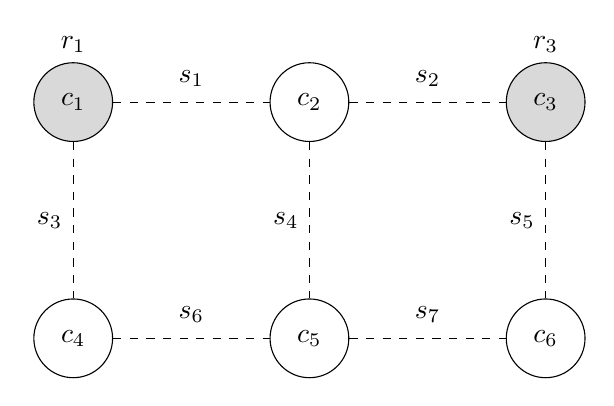
\begin{tikzpicture}[x=1.5cm,y=1.5cm]

 % 設定
 \tikzset{root/.style={circle,draw=black,fill=gray!30,minimum size=1cm}}
 \tikzset{node/.style={circle,draw=black,minimum size=1cm}}
 
 % 補助線
 % \draw [help lines,blue,step=2cm] (-3,0) grid (3,-3);

 % root %
 \node[root] at (-2,0) (1){$c_1$};
 \node[above=0.5cm] at (1) {$r_1$};
 \node[root] at (2,0) (3){$c_3$};
 \node[above=0.5cm] at (3) {$r_3$};

 % node %
 \node[node] at (0,0) (2){$c_2$};
 \node[node] at (-2,-2) (4){$c_4$};
 \node[node] at (0,-2) (5){$c_5$};
 \node[node] at (2,-2) (6){$c_6$};

 % 繋がっていない辺は破線
 \foreach \u / \v in {2/3, 2/5, 4/5}
 \draw [dashed] (\u) -- (\v);
 % 繋がってる辺は実線
 \foreach \u / \v in {1/2, 1/4, 3/6, 5/6}
 \draw [dashed] (\u) -- (\v);

 % スイッチ switch %
 \node at (-1,0.2) {$s_1$};
 \node at (1,0.2) {$s_2$};
 \node at (-2.2,-1) {$s_3$};
 \node at (-0.2,-1) {$s_4$};
 \node at (1.8,-1) {$s_5$};
 \node at (-1,-1.8) {$s_6$};
 \node at (1,-1.8) {$s_7$};
 %

\end{tikzpicture}

%%%%%%%%%%%%%%%%%%%%%%%%%%%%%%%%%%%%%%%%%%%%%%%%%%%%%%%%%%
%%% Local Variables:
%%% mode: japanese-latex
%%% TeX-master: paper.tex
%%% End:
}
 \caption{配電網(図\ref{fig:dnet})を表すグラフ}
 \label{fig:dnetgraph}
\end{figure}
%%%%%%%%%%%%%%%%%%%%%%%%%

図\ref{fig:dnet}における需要家$\{c_1,\ldots,c_6\}$は,\textbf{ノード}に対応し,
スイッチ$\{s_1,\ldots,s_7\}$は,\textbf{辺}に対応している.
図中の色付きノード$\{c_1,c_3\}$は変電所と直接繋がっている需要家を意味しており,
\textbf{根}を表している.
また,根はノードの添字を用いて$\{r_1,r_3\}$のように表す.

\comment{ここまで追加しました.}

\theoremstyle{definition}
\newtheorem*{definition*}{定義}

根付き全域森は以下のように定義される~\cite{Minato:dnet:netuki}.
\begin{definition*}
  グラフ$G=(V,E)$と,根と呼ばれる$V$上のノードの集合が与えられたとする.
  このとき,$G$上の根付き全域森とは,以下の制約を満たす$G$の部分グラフ
  $G'=(V,E'), E' \subseteq E$ である.
  \begin{enumerate}
  \item $G'$はサイクルを持たない.(非閉路制約)
  \item $G'$の各連結成分は,ちょうど1つの根を含む.(根付き連結制約)
  \end{enumerate}
本稿では,与えられたグラフ$G$から,根付き全域森
$G'$を求める部分グラフ探索問題を\textbf{根付き全域森問題}と呼ぶ.
\end{definition*}

%%%%%%%%%%%%%%%%%%%%%%%%%
\begin{figure}[htbp]
  \centering
  \scalebox{0.8}{%%%%%%%%%%%%%%%%%%%%%%%%%%%%%%%%%%%%%%%%%%%%%%%%%%
% 根付き全域森 (第2章で使う)
%%%%%%%%%%%%%%%%%%%%%%%%%%%%%%%%%%%%%%%%%%%%%%%%%%

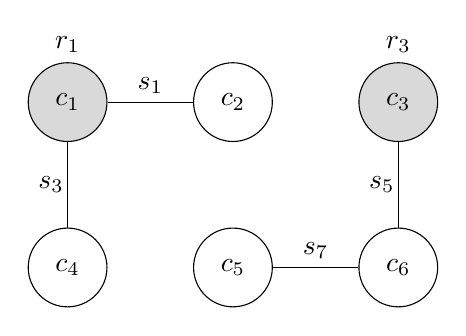
\begin{tikzpicture}[x=1.5cm,y=1.5cm,scale=0.7]

 % 設定
 \tikzset{root/.style={circle,draw=black,fill=gray!30,minimum size=1cm}}
 \tikzset{node/.style={circle,draw=black,minimum size=1cm}}
 
 % 補助線
 % \draw [help lines,blue,step=2cm] (-3,0) grid (3,-3);

 % root %
 \node[root] at (-2,0) (1){$c_1$};
 \node[above=0.5cm] at (1) {$r_1$};
 \node[root] at (2,0) (3){$c_3$};
 \node[above=0.5cm] at (3) {$r_3$};

 % node %
 \node[node] at (0,0) (2){$c_2$};
 \node[node] at (-2,-2) (4){$c_4$};
 \node[node] at (0,-2) (5){$c_5$};
 \node[node] at (2,-2) (6){$c_6$};

 % 繋がっていない辺は破線
 %\foreach \u / \v in {2/3, 2/5, 4/5}
 %\draw [dashed] (\u) -- (\v);
 % 繋がってる辺は実線
 \foreach \u / \v in {1/2, 1/4, 3/6, 5/6}
 \draw (\u) -- (\v);

 % スイッチ switch %
 \node at (-1,0.2) {$s_1$};
 %\node at (1,0.2) {$s_2$};
 \node at (-2.2,-1) {$s_3$};
 %\node at (-0.2,-1) {$s_4$};
 \node at (1.8,-1) {$s_5$};
 %\node at (-1,-1.8) {$s_6$};
 \node at (1,-1.8) {$s_7$};
 %

\end{tikzpicture}

%%%%%%%%%%%%%%%%%%%%%%%%%%%%%%%%%%%%%%%%%%%%%%%%%%%%%%%%%%
%%% Local Variables:
%%% mode: japanese-latex
%%% TeX-master: paper.tex
%%% End:
}\\[1em]
  \scalebox{0.8}{%%%%%%%%%%%%%%%%%%%%%%%%%%%%%%%%%%%%%%%%%%%%%%%%%%
% 根付き全域森 (第2章で使う)
%%%%%%%%%%%%%%%%%%%%%%%%%%%%%%%%%%%%%%%%%%%%%%%%%%

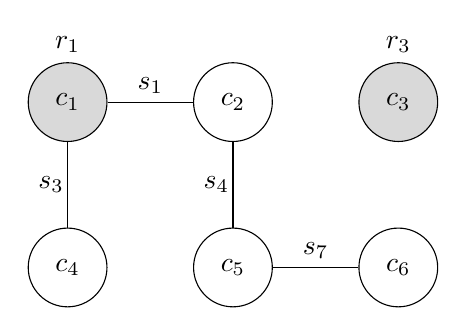
\begin{tikzpicture}[x=1.5cm,y=1.5cm,scale=0.7]

 % 設定
 \tikzset{root/.style={circle,draw=black,fill=gray!30,minimum size=1cm}}
 \tikzset{node/.style={circle,draw=black,minimum size=1cm}}
 
 % 補助線
 % \draw [help lines,blue,step=2cm] (-3,0) grid (3,-3);

 % root %
 \node[root] at (-2,0) (1){$c_1$};
 \node[above=0.5cm] at (1) {$r_1$};
 \node[root] at (2,0) (3){$c_3$};
 \node[above=0.5cm] at (3) {$r_3$};

 % node %
 \node[node] at (0,0) (2){$c_2$};
 \node[node] at (-2,-2) (4){$c_4$};
 \node[node] at (0,-2) (5){$c_5$};
 \node[node] at (2,-2) (6){$c_6$};

 % 繋がっていない辺は破線
 %\foreach \u / \v in {2/3, 2/5, 4/5}
 %\draw [dashed] (\u) -- (\v);
 % 繋がってる辺は実線
 \foreach \u / \v in {1/2, 1/4, 2/5, 5/6}
 \draw (\u) -- (\v);

 % スイッチ switch %
 \node at (-1,0.2) {$s_1$};
 %\node at (1,0.2) {$s_2$};
 \node at (-2.2,-1) {$s_3$};
 \node at (-0.2,-1) {$s_4$};
 %\node at (1.8,-1) {$s_5$};
 %\node at (-1,-1.8) {$s_6$};
 \node at (1,-1.8) {$s_7$};
 %

\end{tikzpicture}

%%%%%%%%%%%%%%%%%%%%%%%%%%%%%%%%%%%%%%%%%%%%%%%%%%%%%%%%%%
%%% Local Variables:
%%% mode: japanese-latex
%%% TeX-master: paper.tex
%%% End:
}
  \caption{根付き全域森の出力例 (2つ)}
  \label{fig:netuki}
\end{figure}
%%%%%%%%%%%%%%%%%%%%%%%%%

根付き全域森の例を図\ref{fig:netuki}に示す.
根付き全域森は,各連結成分が必ずちょうど1つの根をもつ木構造を
形成することで,非閉路制約と根付き連結制約を満たす.
図~\ref{fig:netuki}の上側は,図~\ref{fig:dnet}の配電網問題の解に
対応している.
根付き全域森問題には解が複数存在し得る.
例えば,図~\ref{fig:netuki}の下側は,
ある連結成分が根のみとなる場合を表している.

%%% Local Variables:
%%% mode: japanese-latex
%%% TeX-master: "paper"
%%% End:

\section{解集合プログラミング} \label{chap:asp}

\textbf{解集合プログラミング} (Answer Set Programming; ASP~\cite{%
  Baral03:cambridge,%
  Gelfond88:iclp,%
  Inoue08:jssst,%
  Niemela99:amai})
は,演繹データベース,否定を含む論理プログラミング,
非単調推論,制約充足 (特に,SAT)を起源にもつ,
宣言的プログラミングパラダイムである.
ASP の言語は,一般拡張選言プログラムに基づいている.
本稿では説明の簡略化のため,そのサブクラスである
標準論理プログラムについて説明する.
以降,標準論理プログラムを単に論理プログラムとよぶ.

\textbf{論理プログラム}は,以下の形式をした\textbf{ルール}の有限集合である.
\[
  a_0\leftarrow a_1,\dots,a_m,\naf{a_{m+1}},\dots,\naf{a_n}
\]
ここで,
$0\leq m\leq n$ であり,
各$a_i$はアトム,
$\naf{}$はデフォルトの否定
\footnote{``失敗による否定''ともよばれる.述語論理で定義される否定($\neg$)とは意味が異なる.},
``$,$''は連言を表す.
$\leftarrow$の左側をヘッド,右側をボディとよぶ.
ルールの直観的な意味は,
「$a_1,\ldots,a_m$がすべて成り立ち,$a_{m+1},\ldots,a_n$のそれぞれが成
り立たないならば,$a_0$が成り立つ」である.
ボディが空のルール(すなわち\(a_0\leftarrow\))を\textbf{ファクト}とよび,
$\leftarrow$を省略してよい.

ヘッドが空のルールを\textbf{一貫性制約}とよぶ.
\[
  \leftarrow a_1,\dots,a_m,\naf{a_{m+1}},\dots,\naf{a_n}
\]

直観的には,\(\leftarrow a_1\)は,「$a_1$ではない」という禁止を表し,
\(\leftarrow \naf{a_1}\)は,「$a_1$でなければならない」という強制を表す.
また,
%\(\leftarrow a_1,a_2\)は,「$a_1$と$a_2$が両方同時に成り立つことはない」を意味し,
\(\leftarrow a_1, \naf{a_{2}}\)は,「$a_1$が成り立つならば,$a_2$が成り立つ」を意味する.

ASP 言語は,組合せ問題を解くための便利な拡張構文を備えている.
その代表的なものが\textbf{選択子}と\textbf{個数制約}である.
例えば,選択子\(\{a_1;\dots;a_n\}\)をファクトとして書くと,
「アトム集合\(\{a_1,\dots,a_n\}\)の任意の部分集合が成り立つ」を意味する.
個数制約は選択子の両端に選択可能な個数の上下限を付けたものである.
例えば,\(lb\ \{a_1;\dots;a_n\}\ ub \leftarrow Body\)と書くと,
「$Body$が成り立つならば,$a_1,\dots,a_n$のうち,$lb$個以上$ub$個以下
が成り立つ」を意味する.

\textbf{ASP システム}は,与えられた論理プログラムから,
安定モデル意味論~\cite{Gelfond88:iclp}
に基づく解集合を計算するソフトウェアである.
ASP システムの多くは,
変数を含む論理プログラムを変数を含まない論理プログラムに
\textbf{基礎化}したのち,基礎ソルバーを用いて解集合を計算する.
%近年,SAT ソルバー技術を応用した高速な ASP システムが開発されている.
本稿で使用する高速 ASP システム
{\clingo}~\footnote{\url{https://potassco.org/}}
は,基礎化のためのグラウンダー{\gringo}と基礎ソルバー{\clasp}を
シームレスに結合したものである.
以降で示す論理プログラムのソースコードはすべて{\clingo}言語で書か
れており,表記上の対応については表~\ref{tbl:map}の通りである.

%%%%%%%%%%%%%%%%%%%%%%%%%%%%%%%%%
\begin{table}[t]
  \centering
  \caption{論理プログラムとソースコードの対応}
  \tabcolsep = 2mm
  \begin{tabular}{l|*{5}{c}}\small
    論理プログラム &  $\leftarrow$ & $,$      & $;$      & $\sim$    \\\hline
    ソースコード   &  \code{:-}    & \code{,} & \code{;} & \code{not}
  \end{tabular}
  \label{tbl:map}
\end{table}
%%%%%%%%%%%%%%%%%%%%%%%%%%%%%%%%%
%%%%%%%%%%%%%%%%%%%%%%%%%%%%%%%%%
\lstinputlisting[float=t,caption={%
図~\ref{fig:graph}のグラフの ASP ファクト表現 (\code{graph.lp})},%
captionpos=b,frame=single,label=code:graph.lp,%
xrightmargin=1zw,% 
xleftmargin=1zw,% 
numbersep=5pt,%
numbers=none,%
breaklines=true,%
columns=fullflexible,keepspaces=true,%
basicstyle=\ttfamily\scriptsize]{code/graph.lp}
%%%%%%%%%%%%%%%%%%%%%%%%%%%%%%%%%
%%%%%%%%%%%%%%%%%%%%%%%%%%%%%%%%%
\lstinputlisting[float=t,caption={%
色数 \code{c} のグラフ点彩色問題を解く論理プログラム (\code{color.lp})},%
captionpos=b,frame=single,label=code:color.lp,%
xrightmargin=1zw,% 
xleftmargin=1zw,% 
numbersep=5pt,%
numbers=left,%
breaklines=true,%
columns=fullflexible,keepspaces=true,%
basicstyle=\ttfamily\scriptsize]{code/color.lp}
%%%%%%%%%%%%%%%%%%%%%%%%%%%%%%%%%
%%%%%%%%%%%%%%%%%%%%%%%%%%%%%%%%% 
\lstinputlisting[float=t,caption={%
{\clingo}の実行例},%
captionpos=b,frame=single,label=code:color.log,%
numbers=none,%
breaklines=true,%
columns=fullflexible,keepspaces=true,%
basicstyle=\ttfamily\scriptsize]{code/color.log}
%%%%%%%%%%%%%%%%%%%%%%%%%%%%%%%%%
%%%%%%%%%%%%%%%%%%%%%%%%%%%%%%%%%
\lstinputlisting[float=t,caption={%
基礎化された論理プログラム},%
captionpos=b,frame=single,label=code:color_ground.lp,%
xrightmargin=1zw,% 
xleftmargin=1zw,% 
numbersep=5pt,%
numbers=left,%
breaklines=true,%
columns=fullflexible,keepspaces=true,%
basicstyle=\ttfamily\scriptsize]{code/color_ground.lp}
%%%%%%%%%%%%%%%%%%%%%%%%%%%%%%%%%

ASP を用いた基本的な問題解法は,
最初に解きたい問題を論理プログラムとして表現する.
つぎにASP システムを用いて論理プログラムの解集合を計算する.
最後に解集合を解釈してもとの問題の解を得る,
という3つのステップからなる.
以下,グラフ点彩色問題を例にとって,各ステップごとに説明する.

図~\ref{fig:graph}の無向グラフを,ASP のファクト形式で表したものをコー
ド~\ref{code:graph.lp}に示す.
アトム\code{n/1}は頂点の数,
\code{e/1}は辺の数,
\code{node/1}は頂点,
\code{edge/2}は辺を表している.
ピリオド(``\code{.}'')はルールの終わりを表す終端記号である.

グラフ点彩色問題を解く論理プログラムを,
コード~\ref{code:color.lp}に示す.
コード中の\code{c}は色数を表す定数であり,実際の値は実行時に
{\clingo}のオプションとして与えられる.
1行目のアトム\code{col/1}は色を表し,
\code{col(1..c).}は\code{col(1).}, \code{col(2).}, \ldots,
\code{col(c).}と書くことに等しい.
%
2行目のルールは,頂点\code{X}が色\code{C}で塗られることを意
味するアトム\code{color(X,C)}を導入し,
個数制約を用いて「各頂点は1つの色で塗られる」という制約を表している.
% セミコロン(\code{:})は条件付きリテラ
% ルと呼ばれる拡張構文であり,このルールのヘッドは,
% \code{1 \{ color(X,r);color(X,b);color(X,g) \} 1}のように展開される.
3行目のルールは,一貫性制約と個数制約を使って「辺で結ばれた頂点\code{X}と
\code{Y}が同じ色\code{C}で塗られることはない」という制約を表している.

ASP システムは,
コード~\ref{code:graph.lp}のファクトと
コード~\ref{code:color.lp}の論理プログラム
から解集合を計算する.
コード~\ref{code:color.log}に{\clingo}の実行例を示す.
色\code{1}を赤,色\code{2}を青,色\code{3}を黄とすると,
得られた解集合\{
\code{color(1,1)},
\code{color(2,3)},
\code{color(3,1)},
\code{color(4,2)}\}
は,図~\ref{fig:graph}の右側の彩色を表す.
より詳しく言うと,
{\clingo}は,グラウンダー{\gringo}を用いて
コード~\ref{code:graph.lp}のファクトと
コード~\ref{code:color.lp}の論理プログラムを基礎化した後,
{\clasp}を用いて基礎化された論理プログラムの解集合を計算する.
基礎化されたルール集合をコード~\ref{code:color_ground.lp}に示す.
4--7行目が
コード~\ref{code:color.lp}の2行目に,
8--19行目が
コード~\ref{code:color.lp}の3行目に
対応している.

%%% Local Variables:
%%% mode: japanese-latex
%%% TeX-master: "paper"
%%% End:

\begin{tabular}{l|p{8cm}}
  符号化名 & 遷移制約 \\\hline
  origin & 任意の二つの頂点に対し違反する組合せを列挙することで表現  \\ \hline
  changed & 遷移制約を ASP の個数制約を用いて表現\\\hline
  unchanged & 「各遷移で色が変化しない頂点は$|V|-1$個」という制約を,
         ASPの個数制約を用いて表現
\end{tabular}
%%%%%%%%%%%%%%%%%%%%%%%%%%%%%%%%%%%%%%%%%%%%%%%%%%%%%%%%%% 
\section{実行実験}\label{chap:experiment}
%%%%%%%%%%%%%%%%%%%%%%%%%%%%%%%%%%%%%%%%%%%%%%%%%%%%%%%%%% 

本章では,前章で提案した3つの符号化
\textsf{undirected},\textsf{directed},\textsf{acyclicity}
の性能を評価するために実行実験を行った.
%
実験に使用したベンチマーク問題集(計1008問)は,以下の通りである.
\begin{itemize}
\item \textsf{fhcp} (1001問)\\
  Jerzy Filar と Vladimir Ejov が主導する
  チームプロジェクト Flinders Hamiltonian Cycle Project
  \footnote{\url{https://sites.flinders.edu.au/flinders-hamiltonian-cycle-project/}}
  が提供するハミルトン閉路問題のグラフインスタンス.\cite{haythorpe19:fhcp}
\item \textsf{grid} (6問)\\
  $2N+1$次の正方グリッドグラフのインスタンス($3\leq N\leq 8$).
\item \textsf{usmap} (1問)\\
  図~\ref{fig:USmap}に示されたグラフ.
  D.~E~.Knuth の教科書
  The Art of Computer Programming~\cite{Knuth:TAOCP:SAT}
  に記載されている最短ハミルトン路問題の例.
\end{itemize}

使用した ASP システムは{\clingo}のバージョン5.5.0である.
実験環境は,Mac mini Intel Corei7 3.2GHz 64GBメモリである.

%%%%%%%%%%%%%%%%%%%%%%%%%%%%%%%%%%%%%%%%%%%%%%%%%%%%%%%%%%
\subsection{ハミルトン閉路問題の実験結果}
%%%%%%%%%%%%%%%%%%%%%%%%%%%%%%%%%%%%%%%%%%%%%%%%%%%%%%%%%%

%%%%%%%%%%%%%%%%%%%%%%%%%%%%%%%%%%%%%%%%%%%%%%%
\begin{table}[t]\scriptsize
  \centering
  %\tabcolsep = 0.8mm
  \renewcommand{\arraystretch}{1.2}
  \begin{tabular}{lr|rrr}
    問題サイズ & 問題数 & \textsf{undirected} & \textsf{directed} & \textsf{acyclicity}\\
   \hline
    $\:\:\:\:\:\,\, 0 \leq |V| < 1000$     & 171   & 156   & \alert{171}   & 156  \\ %
    $1000 \leq |V| < 2000$  & 165   & 120   & \alert{159}   & 121  \\
    $2000 \leq |V| < 3000$  & 177   & 125   & \alert{163}   & 80   \\
    $3000 \leq |V| < 4000$  & 185   & 104   & \alert{147}   & 48   \\
    $4000 \leq |V| < 5000$  & 128   & 92    & \alert{106}   & 30   \\
    $5000 \leq |V| < 6000$  & 80    & 63    & \alert{70}    & 21   \\
    $6000 \leq |V| < 7000$  & 55    & 39    & \alert{41}    & 20   \\
    $7000 \leq |V| < 8000$  & 28    & 12    & \alert{15}    & 4    \\
    $8000 \leq |V| < 9000$  & 10    & 2     & \alert{5}     & 1    \\
    $9000 \leq |V| < 10000$  & 2     & \alert{2}     & \alert{2}     & 1    \\
   \hline
    合計 & 1001 & 715   & \alert{879}   & 482  
  \end{tabular}
  \vskip .5em
%  \caption{ハミルトン閉路問題: 解けた問題数}
  \label{sat_table}
\end{table}
%label{sat_table}
%%%%%%%%%%%%%%%%%%%%%%%%%%%%%%%%%%%%%%%%%%%%%%%

%%%%%%%%%%%%%%%%%%%%%%%%%%%%%%%%%%%%%%%%%%%%%%%
\begin{figure}[tb]
\begin{center}
  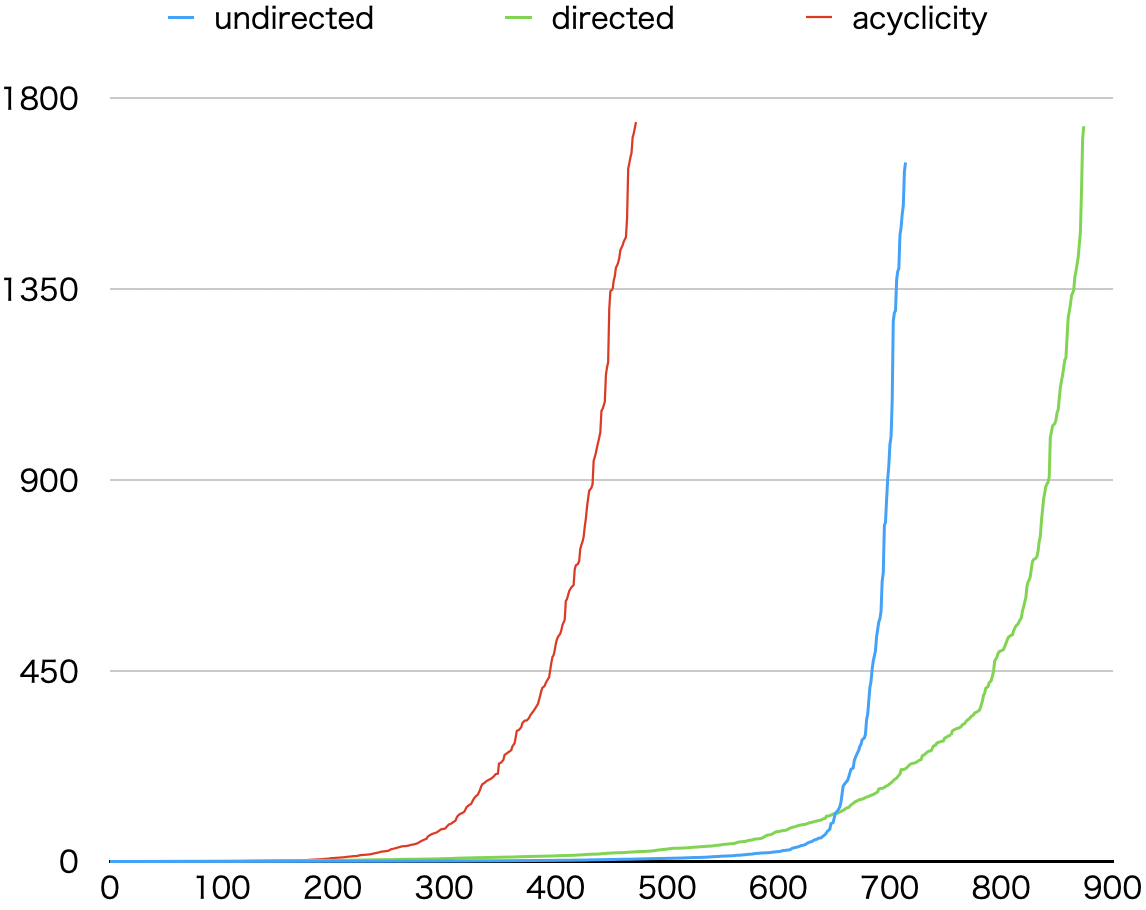
\includegraphics[width=0.8\linewidth]{fig/cactus_fhcp.png}
\caption{ハミルトン閉路問題: カクタスプロット}
\label{cactus}
\end{center}
\end{figure}
%%%%%%%%%%%%%%%%%%%%%%%%%%%%%%%%%%%%%%%%%%%%%%%


%--
本節では,ハミルトン閉路問題の実験結果について述べる.
{\clingo}のオプションは\textit{trendy}を使用し,一問あたりの時間制限を30分とした.
ベンチマーク問題は,\textsf{fhcp}の1001問である.

%--
表~\ref{sat_table}に,各符号化で解けた問題数を,問題の頂点数毎に示す.
左から,問題の頂点数,問題数,各符号化で解けた問題数を示している.
%
解けた問題数は,
\textsf{undirected}符号化が715問,
\textsf{directed}符号化が875問,
\textsf{acyclicity}符号化が473問であり,
\textsf{directed}がもっとも多くの問題を解いた.
\textsf{directed}は,どの頂点数においても同様に,
安定した性能の良さを示した.
図~\ref{cactus}に,カクタスプロットを示す.
縦軸は問題を解くのに要した CPU 時間,横軸は解けた問題数を表す.
グラフが右によるほど多くの問題を解けたことを示し,
下によるほどより速く解けたことを示す.
図~\ref{cactus}より,\textsf{directed}符号化が,
他の2つの符号化と比較して,より多くの問題を高速に解いていることが確認できた.
%% しかし,一部\textsf{undirected}符号化が\textsf{directed}符号化を下回る
%% 部分が確認できる.
%% 実際に,一部の問題では\textsf{undirected}符号化が
%% \textsf{directed}符号化よりも高速に解いていた.

%%%%%%%%%%%%%%%%%%%%%%%%%%%%%%%%%%%%%%%%%%%%%%%%%%%%%%%%%%
\subsection{最短ハミルトン閉路問題}
%%%%%%%%%%%%%%%%%%%%%%%%%%%%%%%%%%%%%%%%%%%%%%%%%%%%%%%%%%

%%%%%%%%%%%%%%%%%%%%%%%%%%%%%%%%%%%%%%%%%%%%%%%
\begin{table}[htbp]
  \caption{実験結果2-1:trendy}
  \label{min_table_tr}
  \centering
  \begin{tabular}{|l|rrr|}
    \hline
    Instance&undirected&directed&acyclicity \\
    \hline
    grid5&50,656*&50,656*&50,656* \\
    grid6&68,656*&68,656*&68,656* \\
    grid7&91,822*&91,822*&91,822* \\
grid8&113,250&\textcolor{red}{112,916}&113,277 \\
grid9&\textcolor{red}{142,502}&143,326&143,660 \\
grid10rc&\textcolor{red}{172,703}&174,866&175,999 \\
grid11&\textcolor{red}{200,399}&204,456&200,638 \\
grid12&\textcolor{red}{231,278}&239,275&232,012 \\
grid13&\textcolor{red}{276,692}&276,926&276,899 \\
grid14&317,617&\textcolor{red}{317,144}&317,676 \\
grid15&\textcolor{red}{375,906}&376,809&376,210 \\
grid16&421,249&\textcolor{red}{419,737}&423,753 \\
US48&11,698*&11,698*&11,698* \\
    \hline
  \end{tabular}
\end{table}
%\label{min_table_tr}
%%%%%%%%%%%%%%%%%%%%%%%%%%%%%%%%%%%%%%%%%%%%%%%

%--
本節では,最短ハミルトン閉路問題の実験結果について述べる.
{\clingo}のオプションは\textit{trendy}を使用し,
一問あたりの時間制限を3時間とした.
ベンチマーク問題は,\textsf{grid}と\textsf{usmap}の合計13問である.

%--
表\ref{min_table_tr}に,各符号化で得られた最適値と最良値を示す.
各問題毎に,最も良かった値を赤字で示している.
*マークは,最適値を表している.
最適値と最良値の数は,
\textsf{undirected}符号化が10問,
\textsf{directed}符号化が7問,
\textsf{acyclicity}符号化が4問であり,
\textsf{undirected}符号化の優位性が確認できた.

%%%%%%%%%%%%%%%%%%%%%%%%%%%%%%%%%%%%%%%%%%%%%%%%%%%%%%%%%%
\subsection{コスト制約付きハミルトン路問題}
%%%%%%%%%%%%%%%%%%%%%%%%%%%%%%%%%%%%%%%%%%%%%%%%%%%%%%%%%%

%%%%%%%%%%%%%%%%%%%%%%%%%%%%%%%%%%%%%%%%%%%%%%%
\begin{table*}[tb]\footnotesize
  \tabcolsep = 2mm
  %\renewcommand{\arraystretch}{1.0}
  \vskip .5em
  \centering
  \begin{tabular}{lr|rrr}
    \hline
    閾値(倍率)    &	解の総数 & \textsf{undirected} & \textsf{directed} & \textsf{acyclicity} \\
    \hline
    11698(1.00)   &	1      &\textbf{2.979} & 7.531 & 4.586	\\
    11814(1.01)   &	8      &5.587  & 15.322	& \textbf{5.250}	\\
    11931(1.02)   &	28     &\textbf{3.243}& 18.600	& 3.578	\\
    12282(1.05)   &	388    &10.003&19.818	& \textbf{6.296}	\\
    12867(1.10)   &	16,180  &16.548& 28.555	& \textbf{9.764}\\
    14037(1.20)   &	939,209 &48.262       &40.717	& \textbf{26.837}\\
    15207(1.30)   &	4,525,541&88.172      &55.276	& \textbf{42.037}\\
    16377(1.40)   &	6,702,964&99.154       &47.647	& \textbf{40.640}	\\
    17547(1.50)   &	6,876,526&95.390       &45.265	& \textbf{38.411}	\\
    18716(1.60)   &	6,876,928&98.937       &49.138	& \textbf{40.748}	\\
    \hline
    平均CPU時間 &   & 46.8275 & 32.7869  & \textbf{21.8147}\\\hline
%    Best    &   & 2 & 0 & \textbf{8} \\ \hline
  \end{tabular}
  \vskip .5em
  \caption{コスト制約付きハミルトン路問題: 解の全列挙に要した CPU 時間}
  \label{cost_table}
\end{table*}
%\label{cost_table}
%%%%%%%%%%%%%%%%%%%%%%%%%%%%%%%%%%%%%%%%%%%%%%%

%--
本節では,第~\ref{chap:background}章でも説明した
コスト制約付きハミルトン路問題(全列挙)の実験結果について述べる.
{\clingo}のオプションは\textit{crafty}を使用し,
一問あたりの時間制限を3時間とした.
ベンチマーク問題は,D.~E~.Knuth の教科書
The Art of Computer Programming~\cite{Knuth:TAOCP:SAT}
に記載されているグラフを使用した(図~\ref{fig:USmap}参照).
このグラフは,米国本土48州の隣接関係を表しており,
頂点数は48,辺の数は105である.
この問題の最短距離は 11698 である(表~\ref{min_table_tr}参照).
今回の実験では,
コスト制約を最短距離のN倍以下
($N=1.00,1.01,1.02,1.05,1.1,1.2,1.3,1.4,1.5,1.6$)として,解の全列挙を
行った.

%--
表~\ref{cost_table}に,各符号化が解の全列挙に要した CPU 時間を示す.
表の1列目はコスト制約の閾値と最短距離からの倍率,2列目は解の総数を表している.
各閾値毎に,最も良かった値を赤字で示している.
表より,
\textsf{acyclicity}符号化が,他の符号化と比較して,より多くの問題を
高速に解いていることがわかる.また,平均CPU時間も最も短い.
%%%%%%%%%%%%%%%%%%%%%%%%%%%%%%%%%%%%%%%%%%%%%%%%%%%%%%%%%%

%%% Local Variables:
%%% mode: latex
%%% TeX-master: "paper"
%%% End:

\chapter{配電網遷移問題への拡張}\label{chap:core}

%%%%%%%%%%%%%%%%%%%%%%%%%%%%%%%%%
\lstinputlisting[float=tb,caption={%
  配電網遷移問題(図~\ref{fig:test-core})のファクト表現},%
captionpos=b,frame=single,label=code:test-core.lp,%
xrightmargin=1zw,% 
xleftmargin=1zw,% 
numbersep=5pt,%
numbers=left,%
breaklines=true,%
columns=fullflexible,keepspaces=true,%
basicstyle=\ttfamily\footnotesize]{code/core-input.lp}
%%%%%%%%%%%%%%%%%%%%%%%%%%%%%%%%%
\lstinputlisting[float=tb,caption={%
  配電網遷移問題のシングルショット符号化},%
captionpos=b,frame=single,label=code:singleshot.lp,%
xrightmargin=1zw,% 
xleftmargin=1zw,% 
numbersep=5pt,%
numbers=left,%
breaklines=true,%
columns=fullflexible,keepspaces=true,%
basicstyle=\ttfamily\small]{code/singleshot.lp}
%%%%%%%%%%%%%%%%%%%%%%%%%%%%%%%%%
\lstinputlisting[float=tb,caption={%
  配電網遷移問題のマルチショット符号化},%
captionpos=b,frame=single,label=code:pw-core.lp,%
xrightmargin=1zw,% 
xleftmargin=1zw,% 
numbersep=5pt,%
numbers=left,%
breaklines=true,%
columns=fullflexible,keepspaces=true,%
basicstyle=\ttfamily\small]{code/pw-core.lp}
%%%%%%%%%%%%%%%%%%%%%%%%%%%%%%%%%

配電網遷移問題は,配電網問題とその2つの実行可能解が与え
られたとき,一方の解(スタート状態)から他方の解(ゴール状態)へ,遷移制約
を満たしつつ,実行可能解のみを経由して最短ステップ長でのスイッチの切替
手順を求める問題である.
各ステップ$t$で切替可能なスイッチの数を$d$個に制限する一般的な
遷移制約を用いる.

本節では,まず,配電網遷移問題インスタンスのASPファクト形式について述べる.
次に,第~\ref{chap:encode}節で示した配電網問題のASP符号化を拡張し,
配電網遷移問題のASP符号化を提案する.
最後に,提案するASP符号化を用いて行った実行実験の結果を示す.

%%%%%%%%%%%%%%%%%%%%%%%%%%%%%%%%%
\textbf{ファクト形式.}
配電網遷移問題は,配電網問題インスタンスに加え,
新たにスタート状態とゴール状態が入力として与えられる.
コード\ref{code:test-core.lp}に,
配電網遷移問題の例(図\ref{fig:test-core})における
スタート状態($t=0$)とゴール状態($t=3$)のファクト表現を示す.
スタート状態における閉じたスイッチは,\code{init_switch/1}によって表される.
また,ゴール状態での閉じたスイッチは,\code{goal_switch/1}によって表される.

%%%%%%%%%%%%%%%%%%%%%%%%%%%%%%%%%
\textbf{シングルショット符号化.}
配電網遷移問題のASP符号化をコード\ref{code:singleshot.lp}に示す.
この符号化は,与えられた配電網遷移問題に対して,ステップ長\code{t}の解が
存在するかを判定し,存在する場合はその解を返す論理プログラムである.
配電網問題のトポロジ制約の有向符号化(コード\ref{code:srf3.lp}),
及び,電流制約のASP符号化(コード\ref{code:electrical.lp})からの拡張点は,
以下の通りである.
\begin{itemize}
 \item 新しくステップを表すアトム\code{t(TT)}を導入.
 \item 制約を表すルールの各アトムにステップを表す項\code{TT}を
       引数として追加.
 \item スタート状態とステップ\code{0},ゴール状態とステップ\code{t}を対応させる
       ルールを追加.
 \item 遷移制約を表すルールを追加.
\end{itemize}
2行目の\code{t(0..t).}は,\code{t(0).},\code{t(1).}, ~... \code{t(t).}に展開され,
各ステップの識別子を表す.定数\code{t}はステップ長を表す整数値であり,
実行時に与えられる.5行目のルールは,スタート状態とステップ\code{0}の閉じたスイッチが
一致することを強制する.同様に,8行目のルールで,ゴール状態とステップ\code{t}の閉じた
スイッチが一致することを強制する.
%
遷移制約は,41--43行目のルールで表される.
\code{changed(SW,t)}は,ステップ\code{t-1}とステップ\code{t}の間でスイッチ\code{SW}
の状態が変化したことを意味する.
43行目のルールで,各ステップ\code{t}において,変化したスイッチの数が\code{d}であること
を保証している.

\textbf{マルチショット符号化.}
シングルショット符号化は, 配電網問題のトポロジ制約と電流制約の符号化の自然な拡張に
なっている.この符号化を用いて遷移問題を解くには,ステップ長\code{t}を増やしながら,
複数の問題を繰り返し解く必要がある.しかし,各問題中の制約の大部分は共通であるため,
ASPシステムが同一の探索空間を何度も調べることになり,求解効率が低下するという問題点
がある.

この問題を解決するために,ASP システム \clingo のマルチショットASP解法を適用する.
この解法は,ASPシステムが同様の探索失敗を避けるために獲得した学習節を(部分的に)
保持することで,無駄な探索を行うことなく,制約を追加した論理プログラムを連続的に
解くことができる.そのため,求解性能の向上が期待できる.

ASPシステム \clingo のマルチショットASP解法ライブラリを用いたASP符号化を
コード\ref{code:pw-core.lp}に示す.
この符号化は,
\code{base},\code{step(t)},\code{check(t)}の3パートから構成される.
%
初めに\code{base}パートには,ステップ\code{t=0}で満たすべき制約を記述する.
ここでは5行目のルールで,スタート状態とステップ\code{0}の対応を記述している.
%
次に\code{step(t)}パートには,各ステップ\code{t}において満たすべき制約を記述する.
ここでは,有向符号化と電流制約の符号化を拡張したルールを記述している(12--39行目).
さらに,42--44行目に遷移制約を表すルールを記述している.
%
最後に,\code{step(t)}パートでは,プログラムの終了条件を記述する.
ここでは,50行目でゴール状態とステップ\code{t}の対応を記述する.
なお,\code{t}がインクリメントされると,一つ前の不要になった終了条件は,\code{query(t)}
の真偽を動的に操作することにより無効化される.

\textbf{実行実験.}
%
DNETで公開されている実用規模の配電網問題
({\sf fukui-tepco},スイッチ数 468,変電所の数 72,$J^{max}=300$)をベースにした.
この問題の実行可能解から,スタート状態を10個,ゴール状態を100個
ランダムに選び,それらを組み合わせた計1000問の配電網遷移問題を生
成し,ベンチマーク問題とした.
実験に用いたASPシステムと実験環境は~\ref{chap:exp}章で示したものと同じである.

シングルショット符号化(コード~\ref{code:singleshot.lp})と,
マルチショット符号化(コード~\ref{code:pw-core.lp})の実行結果を
表~\ref{table:core}に示す.
左から順に,
最短ステップ長,解けた問題数,各符号化の平均CPU時間(秒),シングルショット符号化と
マルチショット符号化の平均CPU時間の比率を示している.
今回行った実行実験では,全てのベンチマーク問題の到達可能性を判定するこ
とができ,すべて到達可能であった.
また,最大で最短ステップ長が7の問題を解くことができた.
マルチショットASP解法を導入することで,通常の解法と比較して,
平均で3.8倍の高速化を実現することができた.

%%%%%%%%%%%%%%%%%%%%%%%%%%%%%%
\begin{table*}[t]
  \centering
  \caption{配電網遷移問題のASP符号化の実行結果}
  \label{table:core}
  \begin{tabular}{ccrrr}
 \rowcolor[RGB]{0,96,0}
\color{white}最短ステップ長 & \color{white}問題数 
     & \multicolumn{1}{c}{\color{white}シングルショット} 
         & \multicolumn{1}{c}{\color{white}マルチショット} 
             & \multicolumn{1}{c}{\color{white}シングル/マルチ} \\
 \rowcolor[RGB]{230,239,230}
1 & 6 & 1.677 & \alert{1.035} & 1.620 \\
 \rowcolor[RGB]{196,230,196}
2 & 62 & 3.507 & \alert{1.608} & 2.180 \\
 \rowcolor[RGB]{230,239,230}
3 & 189 & 6.089 & \alert{2.155} & 2.826 \\
 \rowcolor[RGB]{196,230,196}
4 & 312 & 9.294 & \alert{2.734} & 3.399 \\
 \rowcolor[RGB]{230,239,230}
5 & 280 & 13.338 & \alert{3.361} & 3.968 \\
 \rowcolor[RGB]{196,230,196}
6 & 130 & 18.303 & \alert{4.165} & 4.394 \\
 \rowcolor[RGB]{230,239,230}
7 & 21 & 24.483 & \alert{5.086} & 4.814 \\
\noalign{\hrule height 0.5pt}
 \rowcolor[RGB]{196,230,196}
計 & 1000 & 76.691 & \alert{20.114} & 3.807 \\
\end{tabular}


  %\begin{tabular}{c|c|c|c}
\noalign{\hrule height 1pt}
問題名 & ステップ数$t$ & 問題数 & 平均CPU時間 \\   
\noalign{\hrule height 1pt}
%& 0 & 2 & 0.016 \\
test & 1 & 12 & 0.019 \\
& 2 & 33 & 0.023 \\
& 3 & 64 & 0.026 \\
& 4 & 33 & 0.030 \\
\noalign{\hrule height 1pt}
%0 & 2 & 0.018 \\
baran32 & 1 & 12 & 0.022 \\
& 2 & 66 & 0.027 \\
& 3 & 68 & 0.032 \\
& 4 & 28 & 0.038 \\
\noalign{\hrule height 1pt}
%0 & 2 & 0.508 \\
fukui-tepco & 1 & 11 & 1.012 \\
& 2 & 28 & 1.603 \\
& 3 & 64 & 2.140 \\
& 4 & 38 & 2.724 \\
& 5 & 11 & 3.361 \\
\noalign{\hrule height 1pt}
\end{tabular}

\end{table*}
%%%%%%%%%%%%%%%%%%%%%%%%%%%%%%

%%% Local Variables:
%%% mode: japanese-latex
%%% TeX-master: "paper"
%%% End:


\chapter{おわりに}\label{chap:conc}

本論文では,電気制約として電流制約のみを考慮した配電網問題および配電網
遷移問題に対して,解集合プログラミング(ASP)を用いた解法を提案した.
配電網(遷移)問題に対する ASP を用いた研究は,著者らの知る限り,本論文
がはじめてである.
提案解法の特長と本論文の貢献について,以下にまとめる.

\begin{description}
\item[表現力:]
  配電網問題を解くための ASP 符号化を考案した.
  ASP 言語の高い表現力を生かし,
  配電網問題の制約を簡潔に記述できることを確認した.
  特に,有向符号化は,無向グラフの各辺$u-v$に対して,2つの弧
  $u\rightarrow v$と$v\rightarrow u$を対応させることで有向グラフ化して
  解く符号化であり,非閉路制約を簡潔に表現できる点が特長である.
\item[拡張性:]
  配電網遷移問題に対して,マルチショット ASP 解法を利用した符号化を提案した.
  この符号化は,配電網問題の ASP 符号化の自然な拡張となっている.
  マルチショット ASP 解法を利用することにより,
  ASP システムが同様の探索失敗を避けるために獲得した学習節を
  (部分的に)保持することで,無駄な探索を避けることができる点が特長である.
\item[効率性:]
  DNET (Power Distribution Network Evaluation Tool)
  に公開されている配電網問題(全3問)と,
  Graph Coloring and its Generalizations
  に公開されているグラフを基に独自に生成したトポロジ制約のみの配電網問
  題(計82問)を用いて実行実験を行なった.
  その結果,有向符号化は,他の2つの符号化と比較して,より多くの問題を
  より高速に解くことができ,その優位性を確認できた.
  %
  配電網遷移問題については,実用規模の問題({\sf fukui-tepco})に対して,
  実行可能解のペアをランダムに選び,合計 1000 問の配電網遷移問題を生成
  し,実行実験を行なった.その結果,すべての問題の到達可能性を判定する
  ことができ,得られた最短ステップ長の最大値は7であった.また,
  マルチショットASP解法を導入することにより,
  通常の解法と比較して,平均で3.8倍の高速化を実現した.
\end{description}

今後の課題としては,電流制約と電圧制約を含む完全な配電網問題への拡張が
挙げられる.しかし,完全な問題は非線形な制約を含むため,標準的な ASP
言語では記述できない.この問題を解決するために,近年研究開発が進められ
ている背景理論付き ASP (ASP Modulo Theories~\cite{DBLP:conf/iclp/GebserKKOSW16}) 
を用いた解法の実現可能性について調査を進める.

%%% Local Variables:
%%% mode: japanese-latex
%%% TeX-master: "paper"
%%% End:


\bibliographystyle{jplain}
\bibliography{bachelor,aisat}    % 参考文献リスト

%%%%%%%%%%%%%%%%%%%%%%%%%%%%%%%%%%%%%%%%%%%%%%%%%%%%%%%%%% 
\chapter*{謝辞}
%%%%%%%%%%%%%%%%%%%%%%%%%%%%%%%%%%%%%%%%%%%%%%%%%%%%%%%%%%

本研究を行うにあたり,
研究の着想から論文執筆にわたり
熱心なご指導を頂いた名古屋大学の番原 睦則教授
に深く感謝申し上げます.
また,本研究だけではなく,様々な相談に乗っていただいた
番原研究室の皆様に感謝申し上げます.
最後に,大学生活を通して支えていただいた家族,友人に
感謝申し上げます.


%%% Local Variables:
%%% mode: japanese-latex
%%% TeX-master: "paper"
%%% End:

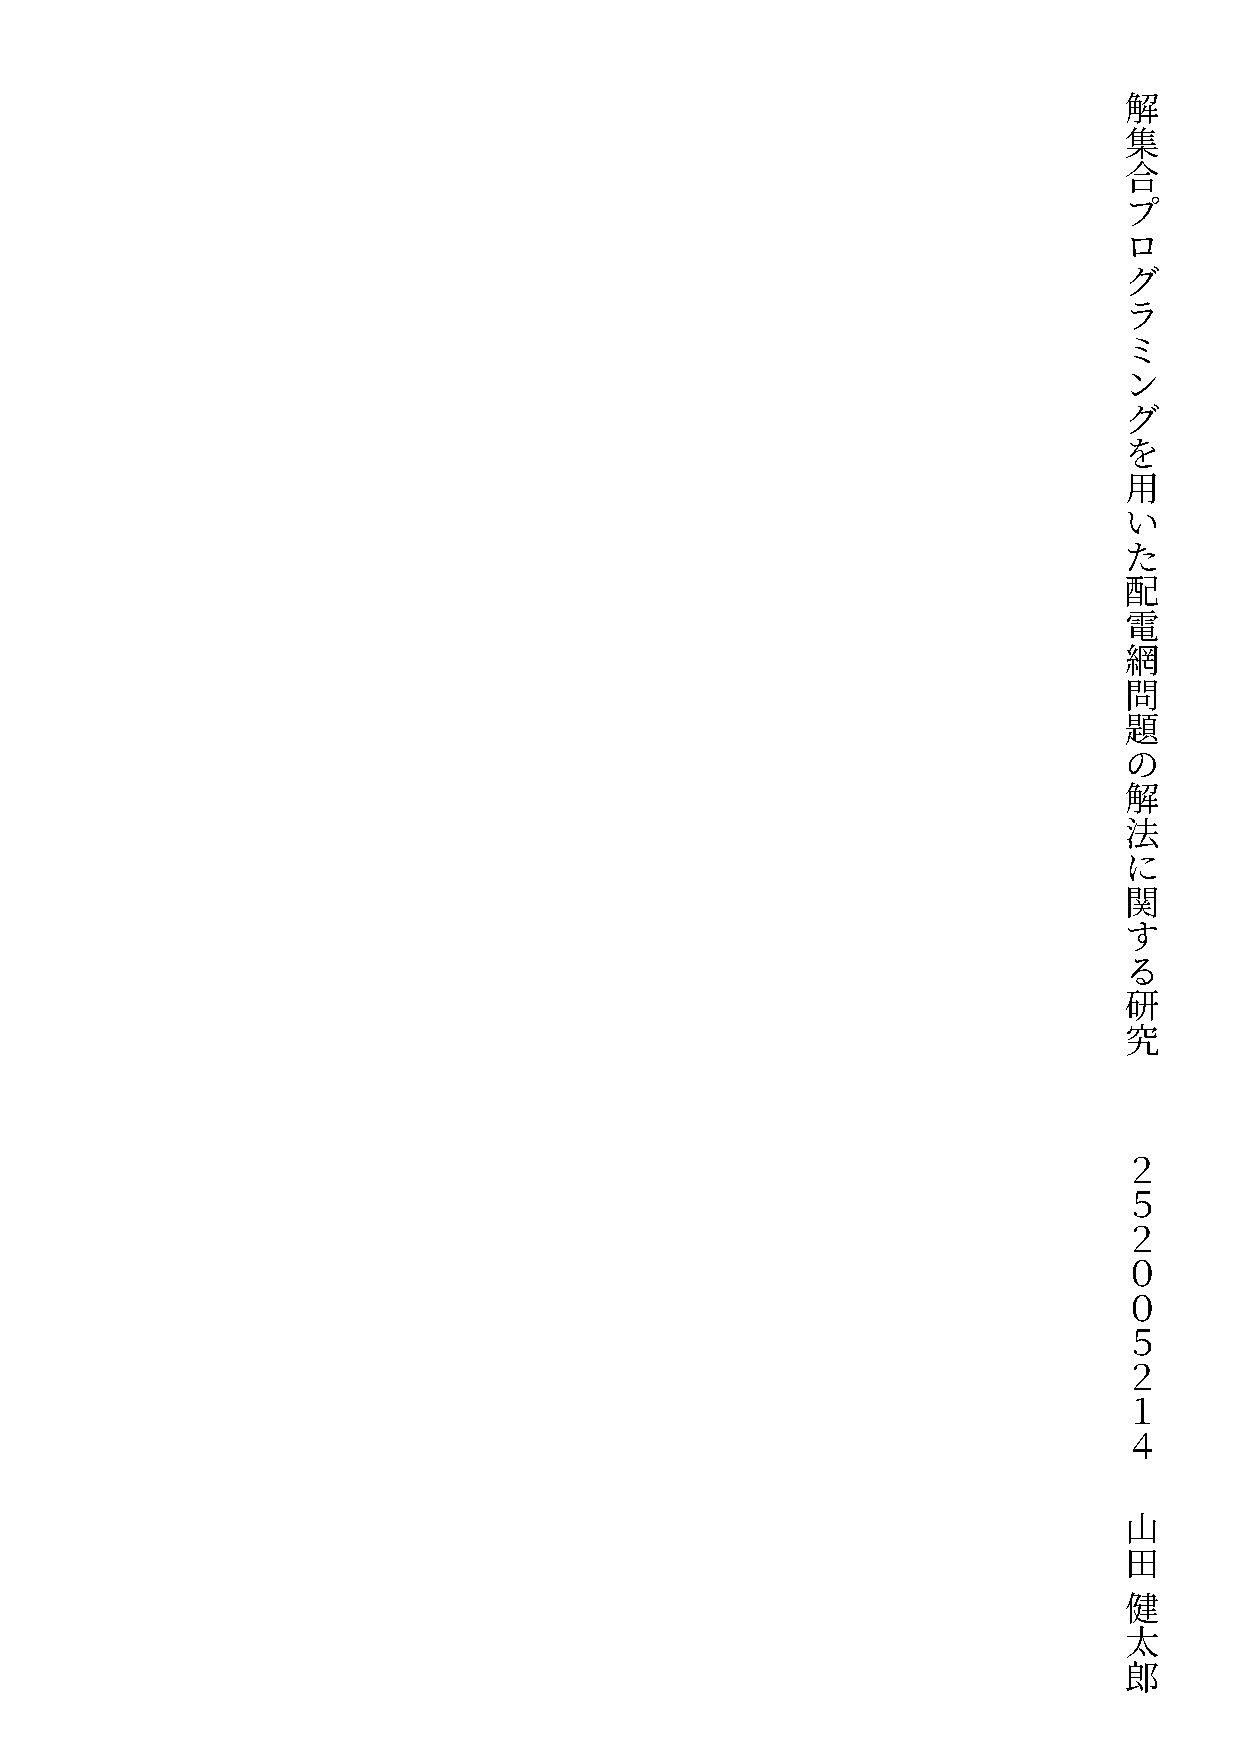
\includepdf{backtitle.pdf}

\end{document}
%%%%%%%%%%%%%%%%%%%%%%%%%%%%%%%%%%%%%%%%%%%%%%%%%%%%%%%%%%

%%% Local Variables:
%%% mode: japanese-latex
%%% TeX-master: t
%%% End:

